% LATeX2e document

\documentclass[12pt]{article}
\pagestyle{empty}

\usepackage{tikz-cd}
\usepackage{amsmath,amssymb,amsfonts,bm}
\usepackage{stmaryrd}
\usepackage{bbold}
\usepackage{times}
\usepackage[all]{xy}
\usepackage{mathrsfs}
\usepackage{graphicx}
\usepackage{url}
\usepackage{pgfplots}
\usepackage{xcolor}
\usepackage{amsthm}
\usepackage[space]{grffile}
\usepackage{float}

\floatstyle{boxed} 
\restylefloat{figure}

\graphicspath{ {C:/Users/Geoffrey/} }
\pgfplotsset{compat=1.12}
\textwidth 1.2\textwidth
\textheight 1.2\textheight
\topmargin 0in
\oddsidemargin 0in
\setlength{\topmargin}{0in}
\setlength{\headsep}{0in}
\setlength{\headheight}{0in}

%%%%%%%%%%%%%%%%%   definitions    %%%%%%%%%%%%%%%%%%%%%%%%%%%%%%%%%%%%

\DeclareMathOperator{\Log}{log}
\DeclareMathOperator{\WN}{WordNorm}
\DeclareMathOperator{\WNt}{WordNormCtrl}
\DeclareMathOperator{\WNp}{WordNormComp}

\newcommand{\onto}{\twoheadrightarrow}
\newcommand{\mono}{\rightarrowtail}
\newcommand{\into}{\hookrightarrow}
\newcommand{\tto}{\longrightarrow}
\newcommand{\iso}{\overset{\sim}{\tto}}
\newcommand{\impl}{\Rightarrow}
\newcommand{\conj}[1]{{}^#1}
\newcommand{\bigslant}[2]{\raisebox{.2em}{$#1$}\left/\raisebox{-.2em}{$#2$}\right.}

\newcommand{\bs}{\mspace{0mu}}
\newcommand{\ednote}[1]{\textcolor{red}{#1}}

\newcommand*{\codefont}{\fontfamily{cmvtt}\selectfont}

%\renewcommand{\labelenumi}{(\alph{enumi})}
\renewcommand{\labelenumi}{\textbf{(\alph{enumi})}}

\definecolor{o5}{RGB}{247,163,46}
\definecolor{o4}{RGB}{249,181,88}
\definecolor{o3}{RGB}{250,200,130}
\definecolor{o2}{RGB}{252,218,171}
\definecolor{o1}{RGB}{253,237,213}
\definecolor{w}{RGB}{255,255,255}
\definecolor{b1}{RGB}{209,213,252}
\definecolor{b2}{RGB}{163,171,250}
\definecolor{b3}{RGB}{116,130,247}
\definecolor{b4}{RGB}{70,88,245}
\definecolor{b5}{RGB}{242,46,242}

\newtheorem{definition}{Definition}

\title{What is the Difference Between Data Science and Machine Learning?}
\date{\today}
\author{Geoffrey E. Schneider}

\begin{document}

\maketitle
\section{Introduction} Data science is the practice of extracting useful information from data. Machine learning is a set of programming techniques in which the programmer sets up a model with variable parameters and a method by which these parameters will be "learned" from data. There. Question answered. In practice, however, when searching for a job, it isn't so clear. Because of the large overlap between the two, a job listed as a data science job may really be more of a machine learning job, and vice versa. And say you want to pick up a few new, relevant skills, but you are primarily interested in one of the two fields. Can we disentangle which skills are more relevant to your chosen field?

The goal of this project is to use textual analysis to distinguish between these two fields. Code is written in the new and exciting programming language Julia. This document was produced using LaTeX \ednote{cite these}.

\section{Data} The data for this project is 150 posted job descriptions. They are divided into three parts, the machine learning descriptions (50), the data science descriptions (50), and the control descriptions (50). These were gathered by doing searches for the relevant words ("machine learning job"/"data science job"/"job"), and then divided into sequences of words using regular expressions. In Julia this is implemented as:

\begin{verbatim} 
function texttowords(text)
  matchall(
    r"(\w+)",
    lowercase(replace(text, r"([\r\n,\.\(\)!;:\?/]|\ufeff)", s" "))
    )
end
\end{verbatim}

The sequences of words were then divided into three "bags of words" (i.e. word counts) for each of the search terms.

\begin{verbatim}
function wordcount(wordvec)
  worddict = Dict{String,Int64}()
  for w in wordvec
    worddict[w]=get(worddict,w,0) + 1
  end
  worddict
end
\end{verbatim} 

\section{WordNorm} To compare two bags of words, we will use two variations on what we will call "WordNorm" (non-technical folks can skip to the tldr at the end if this section, if you want). For word counts $\alpha$ and $\beta$ (e.g. $\alpha = \text{data science}$ and $\beta = \text{control}$) and word $w$, the ideal version of WordNorm
\begin{equation} \label{eqn:WordNorm}
 \WN_{\alpha\beta}(w) = \frac{\alpha(w)-\beta(w)}{\alpha(w)+\beta(w)}.
\end{equation}
We will write $\WN(w)$ when the choice of $\alpha$ and $\beta$ are clear or irrelevant. Note that 
\[
 \WN(w) = \begin{cases} 1 & w \in \alpha \smallsetminus \beta \\ -1 & w \in \beta \smallsetminus \alpha \end{cases}
\]
and that $1$ and $-1$ are the maximum and minimum values of $\WN$. So, if $w$ is near $1$, it is much more closely associated to $\alpha$, and if $w$ is near $-1$, it is much more closely associated to $\beta$. In an ideal setting, with a very large amount of data (so that each word count has at least one of each word), this would work well, however in a practical setting there is an issue. For example, suppose we're interested in comparing the word "dog" to the word "cat", and $\alpha(\text{"dog"}) = 5$, $\alpha(\text{"cat"}) = 1$, but $\beta(\text{"dog"})=\beta(\text{"cat"})=0$. $\WN$ does not distinguish between "dog" and "cat"! $\WN(\text{"dog"})=\WN(\text{"cat"}) = 1$, despite the fact that it is clear that $\alpha$ is probably more strongly associated with "dog" than it is with "cat". To deal with this problem, we will use the two modifications that follow.

When comparing a sample $\alpha$ (e.g. the counts of words in machine learning job descriptions) to a control sample (which we write as $c$) we use
\begin{equation} \label{eqn:WordNormCtrl}
 \WNt_\alpha(w) = \frac{\alpha(w) - (c(w)+1)}{\alpha(w) + (c(w) + 1)}
\end{equation}
where we've written the parentheses to emphasize the interpretation that $\WNt$ is just $\WN$ where we've added one of each word to the control sample. Now using $\beta$ in the example above as a control, we get $\WNt(\text{"dog"})=\frac{2}{3}$ and $\WNt(\text{"cat"})=0$. For our setting $\WNt$ has the nice feature that common words  ("is", "the", etc.) and general job words ("applicant", "responsibilities") get a score close to $0$, and so when we are looking at the top scores, these are automatically ignored. It loses the (anti)symmetry of $\WN$, but this is acceptable, because the sample and control are playing different roles here.

When comparing two samples, we use
\begin{equation} \label{eqn:WordNormComp}
 \WNp_{\alpha\beta}(w) = \frac{\alpha(w) - \beta(w)}{\alpha(w) + \beta(w) +1}.
\end{equation}
This is equivalent to adding half a count of each word to both samples. In a sense, we are saying that we expect that if $\alpha(w)=0$, the "real value" of $\alpha(w)$ is between 0 and 1, but we need a bigger sample to determine the value, so we guess that it is $0.5$, but then to be fair to the other words where $\alpha(w)>0$, we also add $0.5$ to their counts. Here the (anti)symmetry is restored, as it should be since both samples play interchangeable roles. \\
 
\noindent [\textit{tldr: There are a few variations of WordNorm, but in all cases, it assigns a value between 1 and -1 to each word. 1 means the word is much more closely associated to the first bag of words, and -1 means the word is much more closely associated to the second. When one of these is the control, that will always be the second.}]

\section{Results and Discussion} In Figure \ref{fig:WNt} we show the results of applying $\WNt$ to data science (vs. control) and to machine learning (vs. control). We see that the two give broadly similar scores validating the assertion that there is much overlap between the two. Languages such as R, Python and Spark, as well as the distributed system framework Hadoop appear in the top 10 for both.

For "visualization" we see a higher data science score, confirming the stronger importance of communicating findings to allow companies to make informed business decisions, whereas the higher machine learning score for "ai" indicates the importance of building automated systems as a product in themselves. The word "academy" appears at first to be strongly associated with data science and strongly dissassociated with machine learning, however, it is an aberration which should be ignored, as it is on this list only because it appeared a very large number of times in one particular data science job description, and not at all in the control and machine learning data.

\begin{figure}[h]
\begin{center}
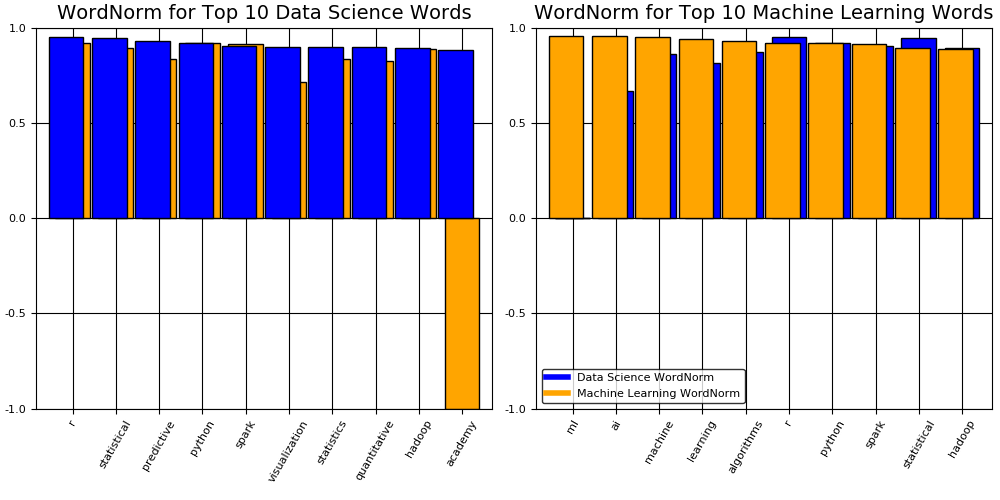
\includegraphics[scale=0.6]{C:/Users/Geoffrey/Documents/Job_descriptions/WordNormTop10.png}
\end{center}
\caption{\label{fig:WNt} The words with the highest $\WNt$ scores for both data science and machine learning.}
\end{figure}

Comparing the data science and machine learning data to the control tells us a lot about what is important to each of them, but due to their large overlap, it does not allow us to \textit{distinguish} them. To do this, we compare them directly using $\WNp$. Figure \ref{fig:WNp} shows the result of applying $\WNp_{ml,ds}$ to directly compare machine learning to data science.

Machine learning frameworks TensorFlow and Caffe are both represented with a stronger association with machine learning whereas words like "consumers" and "audiences" are associated with data science. We also see the names of companies that are associated with machine learning or data science. These company names may be due to the inclusion of jobs advertised by those companies in the dataset, though this is not entirely clear in the case of software companies, where the inclusion may be due to requirements that applicants have knowledge of their software. 

\begin{figure}[h]
\begin{center}
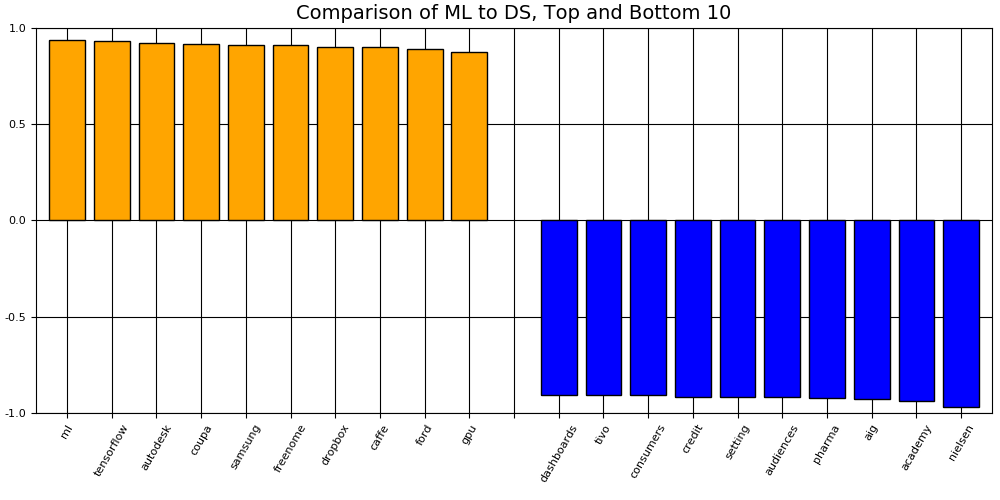
\includegraphics[scale=0.6]{C:/Users/Geoffrey/Documents/Job_descriptions/MLvsDS.png}
\end{center}
\caption{\label{fig:WNp} The result of comparing machine learning to data science with $\WNp$. Positive scores indicate stronger association with machine learning, and negative scores indicate stronger association with data science.}
\end{figure}

Using the $\WNp$ score, we can score any text in terms of whether it is more closely associated with data science or machine learning. For example, the Insight Data Science Fellows Program has a white paper with a section titled "What is a Data Scientist?". We can score this text, word by word, and then average to get a score of -0.13 indicating a closer association with data science than with machine learning.

Figure \ref{fig:InsightColored} shows the first 40 words of this document, each colored according to their $\WNp$ score.

\begin{figure}[H]
the amount of data produced across the globe has been increasing
exponentially and will continue to grow at an accelerating rate for the foreseeable future at companies across all industries servers are overflowing with usage logs message streams transaction records\\

{\color{b1}the} {\color{o1}amount} {\color{b1}of} {\color{b2}data} {\color{w}produced} {\color{b1}across} {\color{b1}the} {\color{b1}globe} {\color{b1}has} {\color{b2}been} {\color{w}increasing} {\color{w}exponentially} {\color{b1}and} {\color{b1}will} {\color{w}continue} {\color{b1}to} {\color{b2}grow} {\color{b1}at} {\color{b1}an} {\color{w}accelerating} {\color{o3}rate} {\color{b1}for} {\color{b1}the} {\color{w}foreseeable} {\color{b2}future} {\color{b1}at} {\color{b3}companies} {\color{b1}across} {\color{b2}all} {\color{w}industries} {\color{w}servers} {\color{b1}are} {\color{w}overflowing} {\color{b1}with} {\color{b1}usage} {\color{w}logs} {\color{o2}message} {\color{o1}streams} {\color{b1}transaction} {\color{w}records}
\caption{\label{fig:InsightColored} The first 40 words of "What is a Data Scientist?" from the Insight Data Science Fellows white paper, first uncolored, then colored according to its $\WNp$ score. Data science associated words are blue, machine learning associated words are in orange, and lighter means closer to 0.}
\end{figure}

\end{document}